\documentclass[letterpaper]{article}
\usepackage[margin=1in]{geometry}
\usepackage{amsmath,amssymb}
\usepackage{tikz}

\newcommand{\aln}[1]{\begin{align*} #1 \end{align*}} % fast align

\begin{document}

\tikzstyle{every node}=[circle, draw, fill=black!50, inner sep=0pt, minimum width=4pt]

\title{Gr\"obner Bases of some Undirected Graphs}
\author{Max Comstock}
\date{Summer 2014}
\maketitle

\section{Three Vertices with One Hamiltonian Cycle}
We will begin by examining a few simple graphs with a single Hamiltonian cycle and varying numbers of vertices. In the case of undirected graphs, we should find that the Gr\"obner basis follow a pattern, although it is more complicated than the pattern for directed graphs with a single Hamiltonian cycle. Our first graph has three vertices:
\begin{center}
  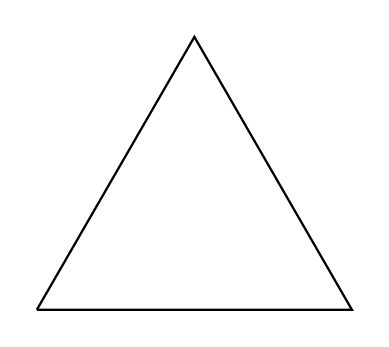
\begin{tikzpicture}[thick,scale=0.8]
    \draw (0,0) node {} -- (5,0) node {} -- (60:5) node {} -- (0,0);
  \end{tikzpicture}
\end{center}
To create a system of polynomial equations for this graph, we treat it as a directed graph with two arcs for each edge of the original graph, one going in each direction. This leads to a more complicated polynomial equation and therefore a more complicated Gr\"obner basis than the simple directed case. For this graph, the system of equations is
\aln{
  z^2 + z + 1 &= 0\\
  x_i^3 - 1 &= 0 \quad 1 \leq i \leq 3\\
  (z x_1 - x_2) (z x_1 - x_3) &= 0\\
  (z x_2 - x_3) (z x_2 - x_1) &= 0\\
  (z x_3 - x_1) (z x_3 - x_2) &= 0
}
By taking the reduced Gr\"obner basis of the ideal generated by these polynomials, we find
\aln{
  %\{x_3^3-1, x_2z^2+x_2z+x_2-x_3z^2-x_3z-x_3, x_2^2+x_2x_3-x_3^2z^2-x_3^2z, x_1+x_2-x_3z^2-x_3z\}
  \{x_3^3-1, x_2^2+x_2x_3+x_3^2, x_1+x_2+x_3\}
}

\newpage

\section{Four Vertices with One Hamiltonian Cycle}
Next, we examine the case with four vertices:
\begin{center}
  \begin{tikzpicture}[thick,scale=0.8]
    \draw (0,0) node {} -- (5,0) node {} -- (5,5) node {} -- (0,5) node {} -- (0,0);
  \end{tikzpicture}
\end{center}
In this case, the graph corresponds to the system of equations
\aln{
  z^2 + 1 &= 0\\
  x_i^4 - 1 &= 0 \quad 1 \leq i \leq 4\\
  (z x_1 - x_2) (z x_1 - x_4) &= 0\\
  (z x_2 - x_3) (z x_2 - x_1) &= 0\\
  (z x_3 - x_4) (z x_3 - x_2) &= 0\\
  (z x_4 - x_1) (z x_4 - x_3) &= 0
}
The reduced Gr\"obner basis of the ideal generated by these polynomials is
\aln{
  %\{&x_4^4-1, x_3^2z^2-x_3^2+x_4^2z^2-x_4^2, x_3^4-1, x_2z^2-x_2+x_4z^2-x_4,\\& x_2x_3-x_2x_4z-x_3^2z+x_3x_4+x_4^2z^3-x_4^2z, x_2^4-1, x_1-x_2z+x_3-x_4z\}
  \{x_4^4-1, x_3^2+x_4^2, x_2+x_4, x_1+x_3\}
}

\newpage

\section{Five Vertices with One Hamiltonian Cycle}
We will now examine a similar graph with five vertices:
\begin{center}
  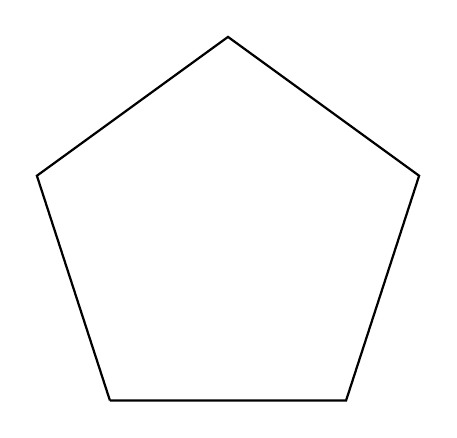
\begin{tikzpicture}[thick,scale=0.6]
    \draw (0,0) node{} -- (5,0) node{} -- ++(72:5) node{} -- ++(2*72:5) node{} -- ++(3*72:5) node{} -- (0,0);
  \end{tikzpicture}
\end{center}
We find that the following system of equations represents the Hamiltonian cycles of the graph:
\aln{
  z^4 + z^3 + z^2 + z + 1 &= 0\\
  x_i^5 - 1 &= 0 \quad 1 \leq i \leq 5\\
  (z x_1 - x_2) (z x_1 - x_5) &= 0\\
  (z x_2 - x_3) (z x_2 - x_1) &= 0\\
  (z x_3 - x_4) (z x_3 - x_2) &= 0\\
  (z x_4 - x_5) (z x_4 - x_3) &= 0\\
  (z x_5 - x_1) (z x_5 - x_4) &= 0
}
The Gr\"obner basis of the ideal generated by these polynomials is
\aln{
  %\{&x_5^5-1, x_4^2z-x_4^2+x_4x_5z^4-x_4x_5z^2+x_4x_5z-x_4x_5+x_5^2z-x_5^2,\\& x_4^5-1, x_3z-x_3+x_4z4-x_4z2+x_4z-x_4+x_5z-x_5,\\& x_3x_4-x_3x_5-x_4^2+2x_4x_5z^4-x_4x_5z3-x_4x_5z^2+2x_4x_5z-x_4x_5+x_5^2z^4+x_5^2z-2x_5^2, x_3^5-1,\\& x_2z-x_2-x_4z^4+x_4z^2-x_4z+x_4-x_5z^4+x_5z2-x_5z+x_5,\\& x_2x_3-x_2x_4-x_3^2+x_3x_5+x_4^2-x_4x_5z^4+x_4x_5z^3+x_4x_5z^2-x_4x_5z-x_4x_5+x_5^2z^4-x_5^2z^3-x_5^2z^2+x_5^2z,\\& x_2^2x_4-x_2^2x_5-x_2x_4^2+x_2x_5^2+x_4^2x_5-x_4x_5^2z^4-x_4x_5^2z+x_4x_5^2-x_5^3z^3-x_5^3z^2+2x_5^3,\\& x_2^5-1, x_1z-x_1+x_4z-x_4+x_5z^4-x_5z^2+x_5z-x_5,\\& x_1x_4-x_1x_5-x_4x_5+x_5^2z^4+x_5^2z-x_5^2,\\& x_1x_3^4+x_1x_3^3x_5+x_1x_3^2x_5^2+x_1x_3x_5^3+x_1x_5^4-x_2x_4^4-x_2x_4^3x_5-x_2x_4^2x_5^2-x_2x_4x_5^3\\& \quad -x_2x_5^4-x_3^4x_5-x_3^3x_5^2-x_3^2x_5^3+4x_3x_5^4+x_4^4x_5+x_4^3x_5^2+x_4^2x_5^3-4x_4x_5^4z^4+x_4x_5^4z^3\\& \quad +x_4x_5^4z^2-4x_4x_5^4z+2x_4x_5^4-z^4-z^3-z^2-z+4,\\& x_1x_2-x_1x_3-x_2^2+x_2x_4+x_3^2-x_3x_5-x_4^2-x_4x_5z^3-x_4x_5z^2+3x_4x_5-x_5^2z^4+x_5^2z^3+x_5^2z^2-x_5^2z,\\& x_1^2-x_1x_3-x_1x_5-x_2^2+x_2x_4+x_2x_5+x_3^2-x_3x_5-x_4^2+2x_4x_5z^4-2x_4x_5z^3-2x_4x_5z^2+2x_4x_5z\\& \quad +x_4x_5+x_5^2z^4+x_5^2z-2x_5^2\}
  \{&x_5^5-1, x_4^2+x_4x_5z^3+x_4x_5z^2+x_4x_5+x_5^2, x_3+x_4z^3+x_4z^2+x_4+x_5,\\& x_2-x_4z^3-x_4z^2-x_4-x_5z^3-x_5z^2-x_5, x_1+x_4+x_5z^3+x_5z^2+x_5\}
}

\newpage

\section{Six Vertices with One Hamiltonian Cycle}
Finally, we extend our previous results to the case with six vertices:
\begin{center}
  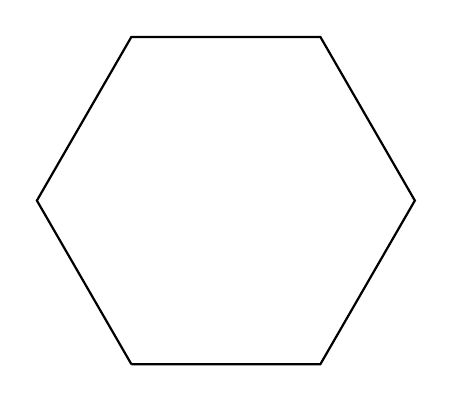
\begin{tikzpicture}[thick,scale=0.6]
    \draw (0,0) node{} -- (4,0) node{} -- ++(60:4) node{} -- ++(2*60:4) node{} -- ++(3*60:4) node{} -- ++(4*60:4) node{} -- (0,0);
  \end{tikzpicture}
\end{center}
In this case, the system of polynomial equations is
\aln{
  z^2 - z + 1 &= 0\\
  x_i^6 - 1 &= 0 \quad 1 \leq i \leq 6\\
  (z x_1 - x_2) (z x_1 - x_6) &= 0\\
  (z x_2 - x_3) (z x_2 - x_1) &= 0\\
  (z x_3 - x_4) (z x_3 - x_2) &= 0\\
  (z x_4 - x_5) (z x_4 - x_3) &= 0\\
  (z x_5 - x_6) (z x_5 - x_4) &= 0\\
  (z x_6 - x_1) (z x_6 - x_5) &= 0
}
The Gr\"obner basis of the ideal generated by these polynomials is
\aln{
  %\{&x_6^6-1, x_5^2z^2-x_5^2+x_5x_6z^5-x_5x_6z3+x_6^2z^2-x_6^2, x_5^6-1, x_4z^2-x_4+x_5z^5-x_5z^3+x_6z^2-x_6,\\& x_4x_5-x_4x_6z-x_5^2z-x_5x_6z^4+x_5x_6z^2+x_5x_6+x_6^2z^5-x_6^2z, x_4^6-1,\\& x_3z^2-x_3-x_6z5+x_6z^3 x_3x_4-x_3x_5z-x_4^2z+x_4x_6z+x_5^2z+2x_5x_6z^4-2x_5x_6z^2-x_5x_6-x_6^2z^5+x_6^2z,\\& x_3^6-1, x_2z^2-x_2-x_5z5+x_5z^3,\\& x_2x_3-x_2x_4z-x_3^2z+x_3x_5z+x_4^2z-x_4x_6z-x_5^2z-2x_5x_6z^4+2x_5x_6z^2+x_5x_6,\\& x_2^2x_5-x_2^2x_6z-x_2x_5^2z+x_2x_6^2z-x_3^2x_5+x_3^2x_6z+x_3x_5^2-x_3x_6^2-2x_5x_6^2z^4+2x_5x_6^2\\& \quad +x_6^3z^3-x_6^3z,\\& x_2^6-1, x_1z^2-x_1+x_5z^2-x_5+x_6z^5-x_6z3,\\& x_1x_5-x_1x_6z-x_5x_6z+x_6^2z^2,\\& x_1x_3^5+x_1x_3^4x_6z+x_1x_3^3x_6^2+x_1x_3^2x_6^3z+x_1x_3x_6^4+x_1x_6^5z-x_2x_4^5-x_2x_4^4x_6\\& \quad -x_2x_4^3x_6^2-x_2x_4^2x_6^3-x_2x_4x_6^4-x_2x_6^5-x_3^5x_6z-x_3^4x_6^2-x_3^3x_6^3z-x_3^2x_6^4\\& \quad +x_3x_5^5+x_3x_5^4x_6z+x_3x_5^3x_6^2+x_3x_5^2x_6^3z+x_3x_5x_6^4+x_4^5x_6+x_4^4x_6^2+x_4^3x_6^3\\& \quad +x_4^2x_6^4-5x_4x_6^5-x_5^5x_6z-x_5^4x_6^2-x_5^3x_6^3z-x_5^2x_6^4+2x_5x_6^5z^5-x_5x_6^5z^3\\& \quad +4x_5x_6^5z+4z^4-2z^2-3,\\& x_1x_2-x_1x_3z-x_2^2z+x_2x_4z+x_3^2z-x_3x_5z-x_4^2z+x_4x_6z+x_5^2z\\& \quad +x_5x_6z^4-x_5x_6z^2-x_5x_6+x_6^2z^5-x_6^2z,\\& x_1^2-x_1x_3-x_1x_6z-x_2^2+x_2x_4+x_2x_6+x_3^2-x_3x_5-x_4^2+x_4x_6+x_5^2-x_5x_6z+x_6^2z^2-x_6^2\}
  \{x_6^6-1, x_5^2-x_5x_6+x_6^2, x_4-x_5+x_6, x_3+x_6, x_2+x_5, x_1+x_5-x_6\}
}

\newpage

\section{Four Vertices with no Hamiltonian Cycles}
We will now move on to a graph with no Hamiltonian cycles. The solution to the polynomial system in this case should have a very different form.
\begin{center}
  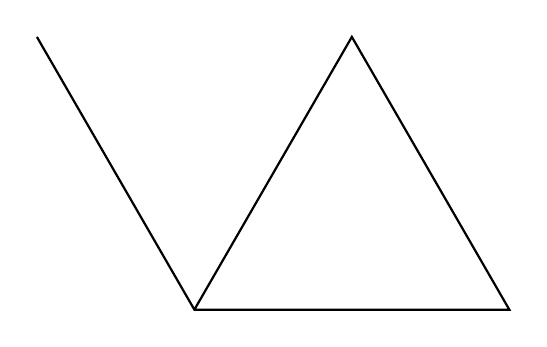
\begin{tikzpicture}[thick,scale=0.8]
    \draw (120:5) node{} -- (0,0) node{} -- (5,0) node{} -- (60:5) node{} -- (0,0);
  \end{tikzpicture}
\end{center}
The system of equations representing the Hamiltonian cycles in this graph is
\aln{
  z^2 + 1 &= 0\\
  x_i^4 - 1 &= 0 \quad 1 \leq i \leq 4\\
  z x_1 - x_2 &= 0\\
  (z x_2 - x_3) (z x_2 - x_4) (z x_2 - x_1) &= 0\\
  (z x_3 - x_4) (z x_3 - x_2) &= 0\\
  (z x_4 - x_2) (z x_4 - x_3) &= 0
}
The Gr\"obner basis of the ideal generated by these polynomials is
\aln{
  %\{x_4^4-1, x_3z+x_3-x_4z-x_4, x_3^2-x_4^2, x_2x_3-x_2x_4z+x_3x_4-x_4^2z, x_2^4-1, x_1-x_2z\}
  \{1\}
}

\newpage

\section{Complete Graph with Four Vertices}
We will now examine the complete four-vertex graph.
\begin{center}
  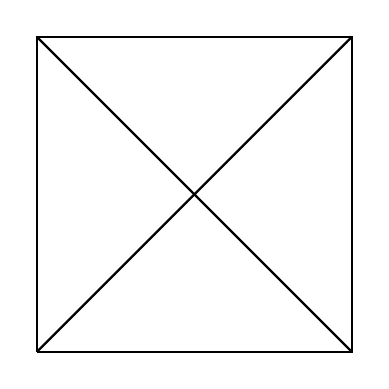
\begin{tikzpicture}[thick,scale=0.8]
    \draw (0,0) -- (5,5);
    \draw (5,0) -- (0,5);
    \draw (0,0) node {} -- (5,0) node {} -- (5,5) node {} -- (0,5) node {} -- (0,0);
  \end{tikzpicture}
\end{center}
In this case, the graph corresponds to the system of equations
\aln{
  z^2 + 1 &= 0\\
  x_i^4 - 1 &= 0 \quad 1 \leq i \leq 4\\
  (z x_1 - x_2) (z x_1 - x_4) (z x_1 - x_3) &= 0\\
  (z x_2 - x_3) (z x_2 - x_1) (z x_2 - x_4) &= 0\\
  (z x_3 - x_4) (z x_3 - x_2) (z x_3 - x_1) &= 0\\
  (z x_4 - x_1) (z x_4 - x_3) (z x_4 - x_2) &= 0
}
The Gr\"obner basis of the ideal generated by these polynomials is
\aln{
  \{x_4^4-1, x_3^3+x_3^2x_4+x_3x_4^2+x_4^3, x_2^2+x_2x_3+x_2x_4+x_3^2+x_3x_4+x_4^2, x_1+x_2+x_3+x_4\}
}

\newpage

\section{Five Vertices with One Hamiltonian Cycle and Additional Edges}
This graph is similar to the previous graph with five vertices, and also has only one cycle. However, it has additional vertices that should not affect the solutions.
\begin{center}
  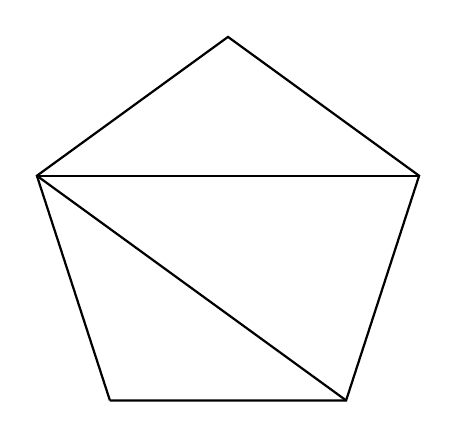
\begin{tikzpicture}[thick,scale=0.6]
    \draw (108:5) -- (5,0);
    \draw (5,0) ++(72:5) -- (108:5);
    \draw (0,0) node{} -- (5,0) node{} -- ++(72:5) node{} -- ++(2*72:5) node{} -- ++(3*72:5) node{} -- (0,0);
  \end{tikzpicture}
\end{center}
The system of polynomial equations for this graph is
\aln{
  z^4 + z^3 + z^2 + z + 1 &= 0\\
  x_i^5 - 1 &= 0 \quad 1 \leq i \leq 5\\
  (z x_1 - x_2) (z x_1 - x_3) (z x_1 - x_4) (z x_1 - x_5) &= 0\\
  (z x_2 - x_3) (z x_2 - x_1) &= 0\\
  (z x_3 - x_4) (z x_3 - x_2) (z x_3 - x_1) &= 0\\
  (z x_4 - x_5) (z x_4 - x_3) (z x_4 - x_1) &= 0\\
  (z x_5 - x_1) (z x_5 - x_4) &= 0
}
The Gr\"obner basis of the ideal generated by these polynomials is
\aln{
 \{&x_5^5-1, x_4^2+x_4x_5z^3+x_4x_5z^2+x_4x_5+x_5^2, x_3+x_4z^3+x_4z^2+x_4+x_5,\\& x_2-x_4z^3-x_4z^2-x_4-x_5z^3-x_5z^2-x_5, x_1+x_4+x_5z3+x_5z2+x_5\}
}

\newpage

\section{Five Vertices with Multiple Hamiltionian Cycles}
Now we will examine some graphs with multiple Hamiltonian cycles. We begin with a graph with five vertices:
\begin{center}
  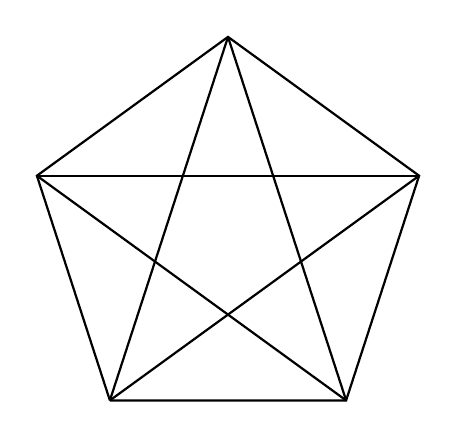
\begin{tikzpicture}[thick,scale=0.6]
    \draw (5,0)++(72:5) -- (0,0);
    \draw (5,0)++(72:5)++(2*72:5) -- (0,0);
    \draw (5,0)++(72:5)++(2*72:5) -- (5,0);
    \draw (108:5) -- (5,0);
    \draw (5,0) ++(72:5) -- (108:5);
    \draw (0,0) node{} -- (5,0) node{} -- ++(72:5) node{} -- ++(2*72:5) node{} -- ++(3*72:5) node{} -- (0,0);
  \end{tikzpicture}
\end{center}
The system of equations for this graph is
\aln{
  z^4 + z^3 + z^2 + z + 1 &= 0\\
  x_i^5 - 1 &= 0 \quad 1 \leq i \leq 5\\
  (z x_1 - x_2) (z x_1 - x_3) (z x_1 - x_4) (z x_1 - x_5) &= 0\\
  (z x_2 - x_1) (z x_2 - x_3) (z x_2 - x_4) (z x_2 - x_5) &= 0\\
  (z x_3 - x_1) (z x_3 - x_2) (z x_3 - x_4) (z x_3 - x_5) &= 0\\
  (z x_4 - x_1) (z x_4 - x_2) (z x_4 - x_3) (z x_4 - x_5) &= 0\\
  (z x_5 - x_1) (z x_5 - x_2) (z x_5 - x_3) (z x_5 - x_4) &= 0
}
The Gr\"obner basis of the ideal generated by these polynomials is

\newpage

\section{Six Vertices with Multiple Hamiltonian Cycles (4-Regular)}
We will now examine a graph with multiple Hamiltonian cycles that has six vertices:
\begin{center}
  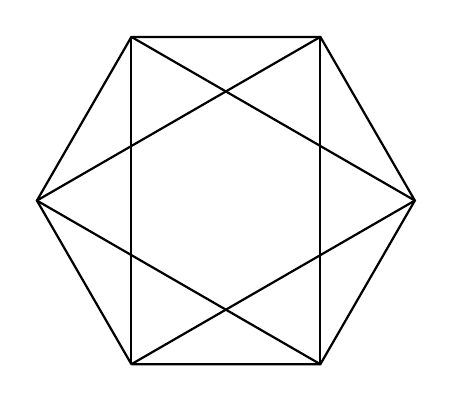
\begin{tikzpicture}[thick,scale=0.6]
    \draw (4,0)++(60:4) -- (0,0);
    \draw (4,0)++(60:4)++(2*60:4)++(3*60:4) -- (0,0);
    \path (4,0)++(60:4)++(2*60:4)++(3*60:4) coordinate(farpoint);
    \draw (4,0)++(60:4) -- (farpoint);
    \draw (4,0)++(60:4)++(2*60:4) -- (4,0);
    \draw (4,0)++(60:4)++(2*60:4) -- (120:4);
    \draw (120:4) -- (4,0);
    \draw (0,0) node{} -- (4,0) node{} -- ++(60:4) node{} -- ++(2*60:4) node{} -- ++(3*60:4) node{} -- ++(4*60:4) node{} -- (0,0);
  \end{tikzpicture}
\end{center}
This graph gives us the system of equations:
\aln{
  z^2 - z + 1 &= 0\\
  x_i^6 - 1 &= 0 \quad 1 \leq i \leq 6\\
  (z x_1 - x_2) (z x_1 - x_3) (z x_1 - x_5) (z x_1 - x_6) &= 0\\
  (z x_2 - x_1) (z x_2 - x_3) (z x_2 - x_4) (z x_2 - x_6) &= 0\\
  (z x_3 - x_1) (z x_3 - x_2) (z x_3 - x_4) (z x_3 - x_5) &= 0\\
  (z x_4 - x_2) (z x_4 - x_3) (z x_4 - x_5) (z x_4 - x_6) &= 0\\
  (z x_5 - x_1) (z x_5 - x_3) (z x_5 - x_4) (z x_5 - x_6) &= 0\\
  (z x_6 - x_1) (z x_6 - x_2) (z x_6 - x_4) (z x_6 - x_5) &= 0
}

\newpage

\section{Six Vertices with Multiple Hamiltonian Cycles (5-Regular)}
Finally, we will examine a graph similar to the previous graph, but with more edges so it is a complete graph.
\begin{center}
  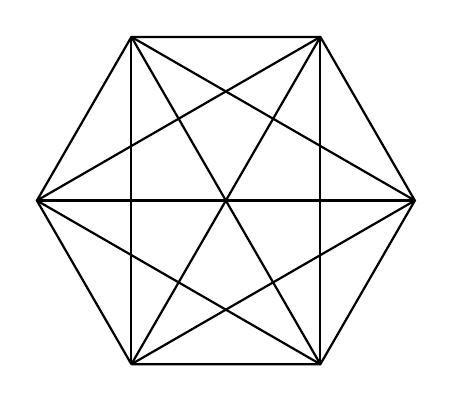
\begin{tikzpicture}[thick,scale=0.6]
    \draw (4,0)++(60:4) -- (0,0);
    \draw (4,0)++(60:4)++(2*60:4)++(3*60:4) -- (0,0);
    \path (4,0)++(60:4)++(2*60:4)++(3*60:4) coordinate(farpoint);
    \draw (4,0)++(60:4) -- (farpoint);
    \draw (4,0)++(60:4)++(2*60:4) -- (4,0);
    \draw (4,0)++(60:4)++(2*60:4) -- (120:4);
    \draw (120:4) -- (4,0);
    \draw (4,0)++(60:4)++(2*60:4) -- (0,0);
    \draw (4,0)++(60:4) -- (120:4);
    \draw (4,0)++(60:4)++(2*60:4)++(3*60:4) -- (4,0);
    \draw (0,0) node{} -- (4,0) node{} -- ++(60:4) node{} -- ++(2*60:4) node{} -- ++(3*60:4) node{} -- ++(4*60:4) node{} -- (0,0);
  \end{tikzpicture}
\end{center}
This graph gives us the system of equations:
\aln{
  z^2 - z + 1 &= 0\\
  x_i^6 - 1 &= 0 \quad 1 \leq i \leq 6\\
  (z x_1 - x_2) (z x_1 - x_3) (z x_1 - x_4) (z x_1 - x_5) (z x_1 - x_6) &= 0\\
  (z x_2 - x_1) (z x_2 - x_3) (z x_2 - x_4) (z x_2 - x_5) (z x_2 - x_6) &= 0\\
  (z x_3 - x_1) (z x_3 - x_2) (z x_3 - x_4) (z x_3 - x_5) (z x_3 - x_6) &= 0\\
  (z x_4 - x_1) (z x_4 - x_2) (z x_4 - x_3) (z x_4 - x_5) (z x_4 - x_6) &= 0\\
  (z x_5 - x_1) (z x_5 - x_2) (z x_5 - x_3) (z x_5 - x_4) (z x_5 - x_6) &= 0\\
  (z x_6 - x_1) (z x_6 - x_2) (z x_6 - x_3) (z x_6 - x_4) (z x_6 - x_5) &= 0
}


\end{document}
